\documentclass[12pt, titlepage]{article}
\usepackage{graphicx}
\usepackage{float}
\restylefloat{table}

% Imported Packages
%------------------------------------------------------------------------------
\usepackage{amssymb}
\usepackage{amstext}
\usepackage{amsthm}
\usepackage{amsmath}
\usepackage{enumerate}
\usepackage{fancyhdr}
\usepackage[margin=1in]{geometry}
\usepackage{graphicx}
\usepackage{extarrows}
\usepackage{setspace}
%------------------------------------------------------------------------------

% Header and Footer
%------------------------------------------------------------------------------
\pagestyle{plain}  
\renewcommand\headrulewidth{0.4pt}                                      
\renewcommand\footrulewidth{0.4pt}                                    
%------------------------------------------------------------------------------

% Title Details
%------------------------------------------------------------------------------
\title{SE 3A04: Software Design III: Large System Design}
\author{Group \#5, Spaceship System Sabotage %Alliteration; always adored and absolutely amazing
		\\Pareek Ravi 001407109
		\\Pavle Arezina 001410366
		\\David Hobson 001412317
		\\Victoria Graff 001401451
		\\Julian Cassano 001406891
}
\date{\today}                          
%------------------------------------------------------------------------------

% Document
%------------------------------------------------------------------------------
\begin{document}

\maketitle	
\pagenumbering{arabic}
\tableofcontents
\listoftables
\listoffigures
\newpage

\section{Introduction}
\label{sec:introduction}
% Begin Section

This section should provide an brief overview of the entire document.

\subsection{Purpose}
\label{sub:purpose}
% Begin SubSection
\begin{enumerate}[a)]
	\item Delineate the purpose of the document
	\item Specify the intended audience for the document
\end{enumerate}
% End SubSection

\subsection{System Description}
\label{sub:system_description}
% Begin SubSection
\begin{enumerate}[a)]
	\item Give a brief description of the system. This could be a paragraph or two to give some context to this document.
\end{enumerate}
% End SubSection

\subsection{Overview}
\label{sub:overview}
% Begin SubSection
\begin{enumerate}[a)]
	\item Describe what the rest of the document contains 
	\item Explain how the document is organised
\end{enumerate}

% End SubSection

% End Section

\section{State Charts for Controller Classes}
\label{sec:state_charts_for_controller_classes}

% Begin Section
\subsection{Tool Controller}
\begin{figure}[H]
\centering
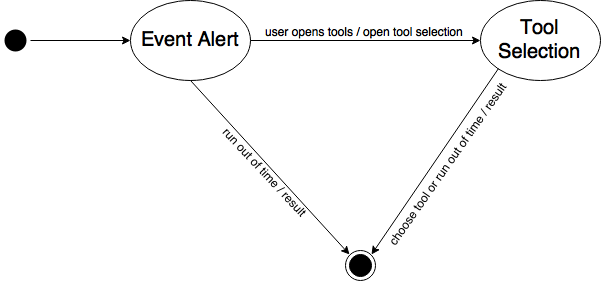
\includegraphics[width=120mm]{ToolController.png}
\caption{Tool Controller State Chart}
\end{figure}

\subsection{Control Object}
\begin{figure}[H]
\centering
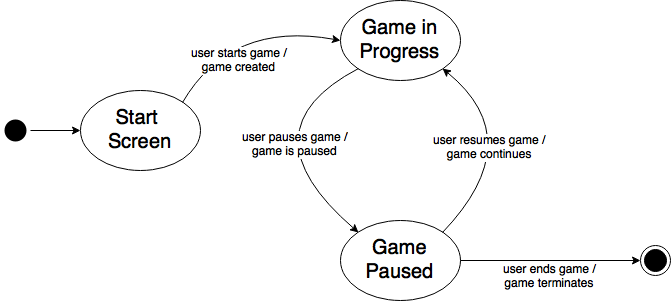
\includegraphics[width=120mm]{ControlObject.png}
\caption{Tool Controller State Chart}
\end{figure}

\subsection{Power Controller}
\begin{figure}[H]
\centering
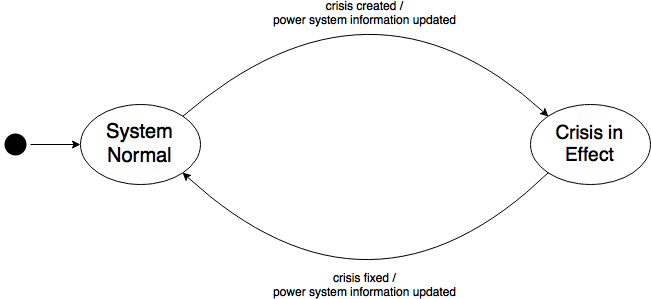
\includegraphics[width=120mm]{PowerController.png}
\caption{Power Controller State Chart}
\end{figure}

\subsection{Mechanical Controller}
\begin{figure}[H]
\centering
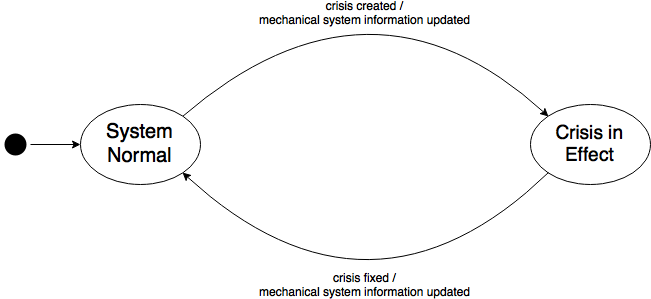
\includegraphics[width=120mm]{MechanicalController.png}
\caption{Mechanical Controller State Chart}
\end{figure}

\subsection{Oxygen Controller}\begin{figure}[H]
\centering
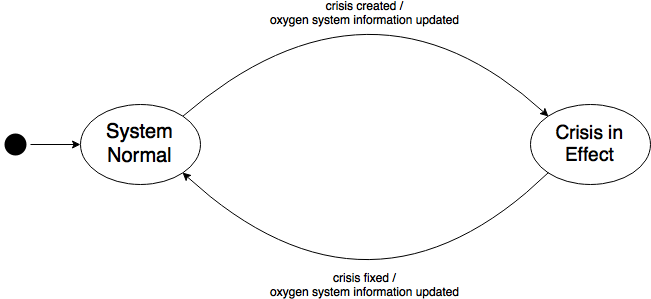
\includegraphics[width=120mm]{OxygenController.png}
\caption{Oxygen Controller State Chart}
\end{figure}

\subsection{Overall Controller}
% End Section

\section{Sequence Diagrams}
\label{sec:sequence_diagrams}
\subsection*{Start Simulation}
\begin{figure}[H]
\centering
\includegraphics[scale = 0.5]{"Start Simulation".jpg}
\caption{Start Simulation Sequence Diagram}
\end{figure}
\subsection*{End Simulation}
\begin{figure}[H]
\centering
\includegraphics[scale = 0.5]{"Stop Simulation".jpg}
\caption{End Simulation Sequence Diagram}
\end{figure}
\subsection*{Pause Simulation}
\begin{figure}[H]
\centering
\includegraphics[scale = 0.5]{"Pause Simulation".jpg}
\caption{Pause Simulation Sequence Diagram}
\end{figure}
\subsection*{Resume Simulation}
\begin{figure}[H]
\centering
\includegraphics[scale = 0.5]{"Resume Simulation".jpg}
\caption{Resume Simulation Sequence Diagram}
\end{figure}
\subsection*{View Overall Simulation}
\begin{figure}[H]
\centering
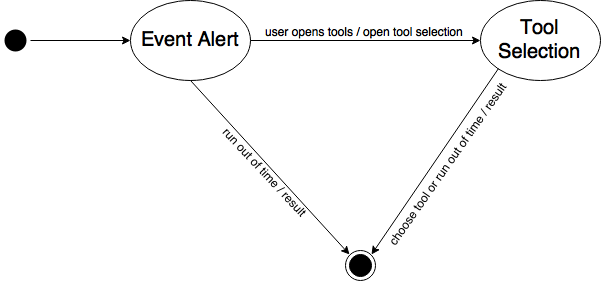
\includegraphics[width=120mm]{ToolController.png}
\caption{Tool Controller State Chart}
\end{figure}
\subsection*{View Power System}
\begin{figure}[H]
\centering
\includegraphics[scale = 0.5]{"View Power System".jpg}
\caption{View Power System Sequence Diagram}
\end{figure}
\subsection*{View Oxygen System}
\begin{figure}[H]
\centering
\includegraphics[scale = 0.5]{"View Electrical System".jpg}
\caption{View Oxygen System Sequence Diagram}
\end{figure}
\subsection*{View Mechanical System}
\begin{figure}[H]
\centering
\includegraphics[scale = 0.5]{"View Mechanical System".jpg}
\caption{View Mechanical System Sequence Diagram}
\end{figure}
\subsection*{Fix Crisis}
\begin{figure}[H]
\centering
\includegraphics[scale = 0.5]{"Untitled Diagram (3)".png}
\caption{Fix Crisis Sequence Diagram}
\end{figure}
\subsection*{Fix Power}
\begin{figure}[H]
\centering
\includegraphics[scale = 0.5]{"Untitled Diagram".png}
\caption{Fix Power Sequence Diagram}
\end{figure}
\subsection*{Fix Oxygen}
\begin{figure}[H]
\centering
\includegraphics[scale = 0.5]{"Untitled Diagram (2)".png}
\caption{Fix Oxygen Sequence Diagram}
\end{figure}
\subsection*{Fix Mechanical}
\begin{figure}[H]
\centering
\includegraphics[scale = 0.5]{"Untitled Diagram (1)".png}
\caption{Fix Mechanical Sequence Diagram}
\end{figure}

\section{Detailed Class Diagram}
\label{sec:detailed_class_diagram}
\begin{figure}[H]
\centering
\includegraphics[width=180mm]{"Class Diagram".png}
\caption{Detailed Class Diagram}
\end{figure}
\newpage
\appendix
\section{Division of Labour}
\label{sec:division_of_labour}
% Begin Section
Include a Division of Labour sheet which indicates the contributions of each team member. This sheet must be signed by all team members.
% End Section




\end{document}
%------------------------------------------------------------------------------